% !TeX root = ./main.tex

\chapter{МОРФОМЕТРИЯ ДИНАМИЧЕСКИХ ИЗОБРАЖЕНИЙ И ПЕРСПЕКТИВЫ}

\section{Экспериментальная верификация переносимости между разрешениями и калибровки сертификата}

Вычислительные эксперименты выполнены в воспроизводимой локальной среде Python~3.11 (\texttt{NumPy 2.4.6}, \texttt{SciPy 1.17.1}~[\ref{itm:scipy}], \texttt{scikit-image 0.26.0}~[\ref{itm:skimage}], главное зерно генератора псевдослучайных чисел \texttt{20261122}). На контрольной задаче теплопроводности с аналитическим решением Неймана ($\kappa=0{,}02$, $T=0{,}25$) подтверждён теоретический второй порядок точности в норме $L^2(\Omega)$: при измельчении сетки от $N=81$ до $N=4225$ узлов погрешность убывает в $62{,}2$~раза (с $1{,}038\times 10^{-2}$ до $1{,}668\times 10^{-4}$, наклон $1{,}986$) на регулярных решётках и с $1{,}134\times 10^{-2}$ до $1{,}778\times 10^{-4}$ (наклон $2{,}112$) на возмущённых триангуляциях Делоне, тогда как максимальная по ячейкам дискретная дивергенция дуальных потоков Дональда на случайном облаке Делоне ($N=450$) составляет $3{,}469\times 10^{-18}$ (машинный нуль стандарта IEEE-754).

На рисунке~\ref{fig:field_2d} представлено двумерное визуальное сопоставление эталонного поля $u^*(x,T)$ и прогнозов при переносе параметров с грубой решётки $18\times 18$ на мелкую сетку $54\times 54$ без дообучения: контур фронта \texttt{CDQuad} неотличим от эталона, тогда как фронт дипломной модели AdaCDE замирает около начального положения вследствие вырождения комбинаторного вентиля.

\begin{figure}[htbp]
    \centering
    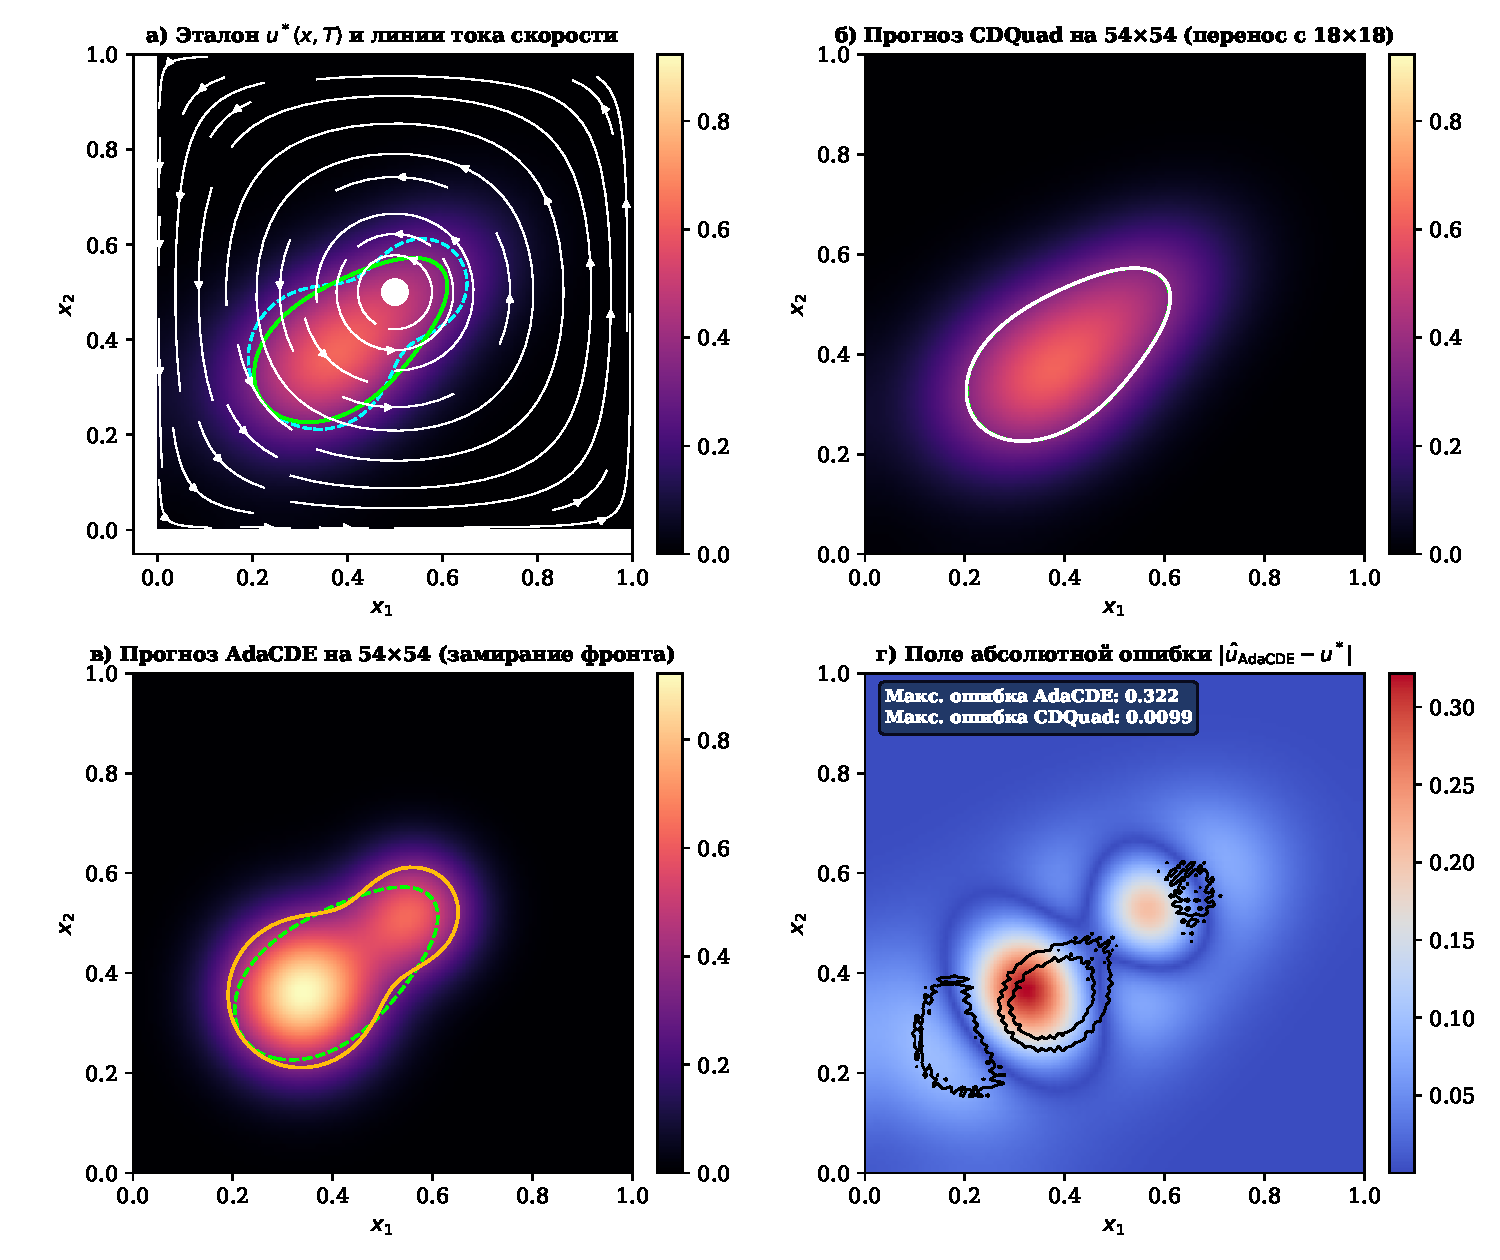
\includegraphics[width=0.94\textwidth]{figures/fig4_field_comparison_2d.pdf}
    \caption{Двумерная визуализация переноса без дообучения с $18\times 18$ на $54\times 54$ ($T=0{,}35$): а)~эталон $u^*(x,T)$ (сплошной контур), начальный контур (пунктир) и линии тока скорости; б)~точный перенос \texttt{CDQuad}; в)~замирание фронта в дипломной AdaCDE; г)~пространственная карта абсолютной ошибки}
    \label{fig:field_2d}
\end{figure}

В серии тестов с вращающейся анизотропией ($\chi(K)=5$) и вихревым переносом при изменении числа Пекле $\Pe\in[0,100]$ расхождение между триангуляциями Делоне $16\times 16$ и $48\times 48$ следует строго линейному закону ($R^2=0{,}9998$, от $0{,}00411$ до $0{,}01513$, рисунок~\ref{fig:peclet_gate}а) при полном отсутствии нефизических осцилляций у противопоточной схемы ($0{,}0$ выбросов за диапазон начальных данных при $\Pe\ge 30$). На длинном горизонте времени $t\in[0,8]$ межуровневая ошибка не накапливается экспоненциально, а монотонно затухает от пикового значения $0{,}00758$ до $0{,}00155$. В противоположность этому у дипломной модели AdaCDE среднее значение локального вентиля падает как $\Theta(n_x^{-2})$ с $0{,}07832$ на сетке $12\times 12$ до $0{,}00399$ на сетке $64\times 64$ (рисунок~\ref{fig:peclet_gate}б).

\begin{figure}[htbp]
    \centering
    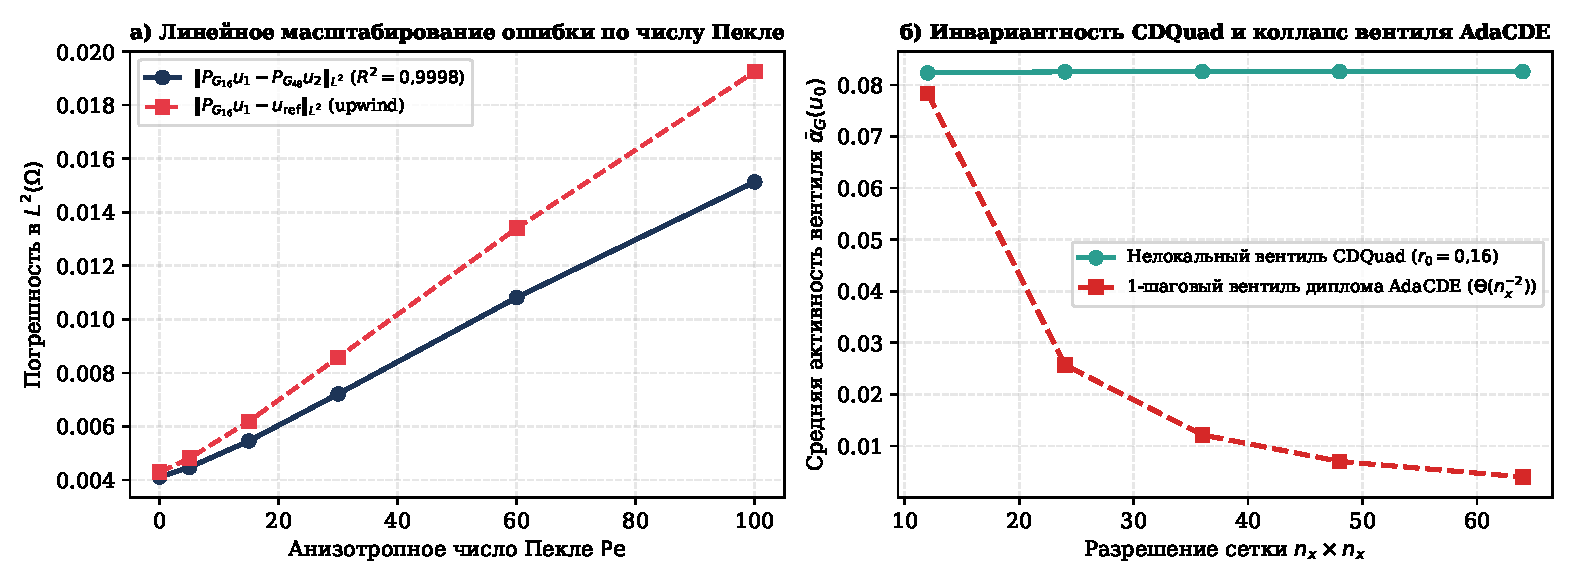
\includegraphics[width=0.98\textwidth]{figures/fig5_peclet_and_gate.pdf}
    \caption{Верификация асимптотических свойств: а)~линейное масштабирование ошибки переноса по числу Пекле; б)~инвариантность континуального вентиля \texttt{CDQuad} против квадратичного вырождения 1-шагового вентиля дипломной AdaCDE}
    \label{fig:peclet_gate}
\end{figure}

Проверка модуля \texttt{src/certificate.py} на $160$ случайных триангуляциях Делоне ($N\in[144,1024]$, $\Pe=35$) показала, что двойственный дефект $\widehat{\delta}_{-1}(G)$ имеет логарифмический наклон по шагу сетки $0{,}992$ и корреляцию с истинной ошибкой переноса $r=0{,}9803$ (против наклона $0{,}242$ и $r=0{,}5590$ у наивного поточечного $L^2$-остатка). При оценке по $200$ случайным перестановочным разбиениям $80/80$ на уровнях надёжности $1-\alpha\in\{0{,}85;\;0{,}90;\;0{,}95\}$ среднее эмпирическое покрытие составило соответственно $0{,}853$, $0{,}902$ и $0{,}953$, при этом нормировка на двойственный дефект сузила ширину доверительных интервалов на $27{,}9\,\%$, $36{,}1\,\%$ и $36{,}5\,\%$ по сравнению с ненормированным конформным предиктором при отношении границы к ошибке $1{,}23\text{--}1{,}30$. На числовом контрпримере подтверждено, что возмущение поля в $L^2(\Omega)$ величиной $0{,}004$ вызывает скачок жёсткой пороговой площади $1{,}0$ (коэффициент усиления $250$), тогда как сглаженная площадь $\calM_0$ при $\eta=0{,}06$ изменяется лишь на $0{,}01667$, точно укладываясь в аналитическую константу Липшица $L_{\calM_0}=4{,}167$. Сводные результаты при $1-\alpha=0{,}90$ и стресс-тестах сдвига распределения сеток приведены в таблице~\ref{tab:cert_table} и на рисунке~\ref{fig:conformal_ood}.

\begin{table}[htbp]
\caption{Верификация конформного сертификата ошибки переноса на случайных триангуляциях и при сдвиге распределения сеток ($1-\alpha=0{,}90$)}\label{tab:cert_table}
\footnotesize
\setlength{\tabcolsep}{4pt}
\renewcommand{\arraystretch}{1.18}
\begin{tabularx}{\textwidth}{@{} Y >{\centering\arraybackslash}p{1.9cm} >{\raggedleft\arraybackslash}p{1.8cm} >{\raggedright\arraybackslash}p{2.9cm} >{\centering\arraybackslash}p{2.2cm} >{\raggedright\arraybackslash}p{2.5cm} @{}}
\toprule
\textbf{Режим тестирования сеток} & \textbf{Выборка} & \textbf{$\bar{e}_{\mathrm{true}}$} & \textbf{Граница $\widehat{U}_{0{,}90}$} & \textbf{Покрытие ($\widehat{\delta}_{-1}$)} & \textbf{Покрытие (конст. CP)} \\
\midrule
Случайные сетки Делоне ID (200 разб.) & 80 / 80 & 0,00644 & 0,00792 ($-36{,}1\%$) & $0{,}902\pm 0{,}046$ & 0,938 (шир. 0,0124) \\
Анизотропное растяжение OOD ($x_1=s^3$) & 30 тест. & 0,01626 & 0,02143 (автомасштаб) & \textbf{1,000} & 0,067 (срыв) \\
Графы суперпикселей SLIC ($K\in[180,480]$) & 30 тест. & 0,02796 & 0,05185 (сигнал RAG) & \textbf{1,000} & 0,000 (срыв) \\
Локальное «слепое пятно» (удалено $94\%$) & 30 тест. & 0,02644 & 0,00938 (недооценка) & 0,000 (граница) & 0,200 (срыв) \\
\bottomrule
\end{tabularx}
\end{table}

\begin{figure}[htbp]
    \centering
    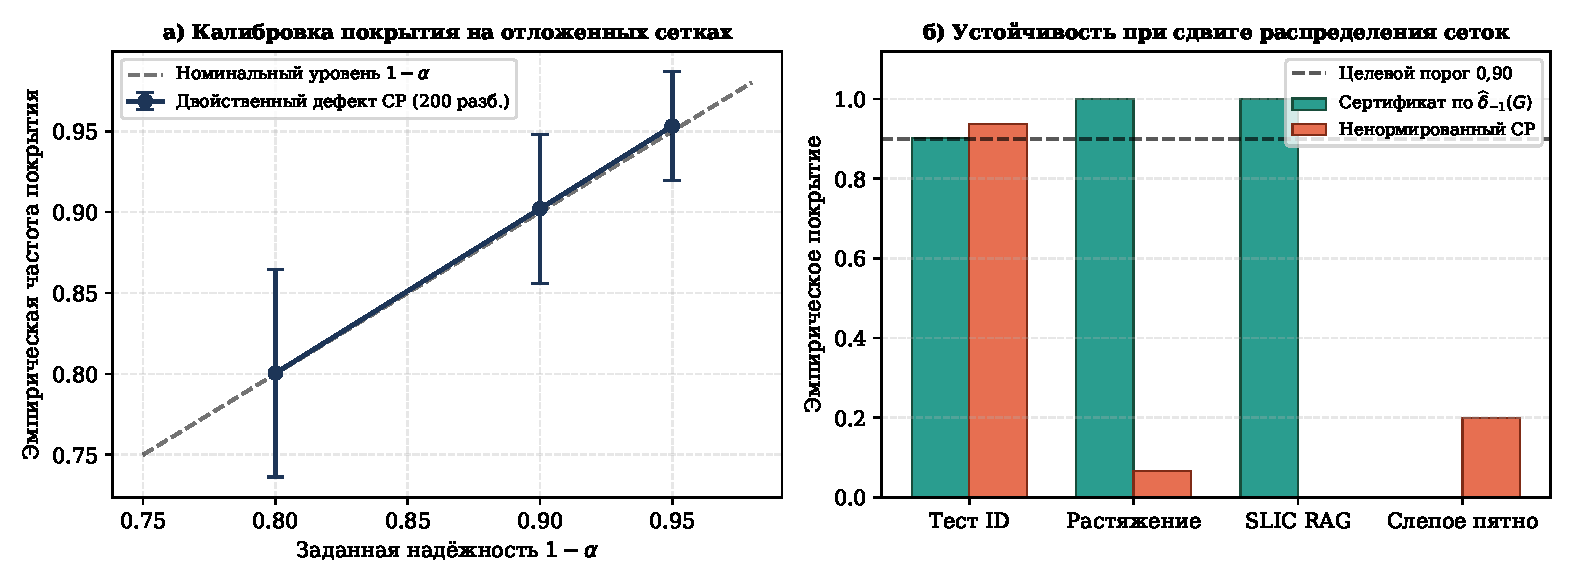
\includegraphics[width=0.98\textwidth]{figures/fig6_conformal_ood.pdf}
    \caption{Проверка статистического сертификата: а)~совпадение эмпирического и номинального покрытия на перестановочных сетках; б)~сохранение покрытия при глобальном растяжении и на SLIC и срыв при локальном «слепом пятне» датчика}
    \label{fig:conformal_ood}
\end{figure}

\section{Морфометрия динамических структур в цейтраферной флуоресцентной микроскопии}

Апробация технологии в регламенте биомедицинского анализа изображений научного направления д-ра техн. наук, доцента А.~М.~Недзьведя~[\ref{itm:ablyameyko}, с.~88;~\ref{itm:nedzvedz2012}, с.~104] проведена в двух взаимодополняющих протоколах: 1)~на синтетическом бенчмарке двухкомпонентных мигрирующих клеточных структур (обучение только на $6$ зашумлённых сериях биннинга $18\times 18$ с $\sigma_{\mathrm{noise}}=0{,}004$, затем перенос без дообучения на мелкую решётку $54\times 54$, триангуляцию Делоне $N=1225$ и граф суперпикселей SLIC $K\approx 300$); 2)~на реальной $15$-кадровой цейтраферной записи ядерного транспорта флуоресцентного белка живой клетки \texttt{NPCsingleNucleus.tif} (разрешение $180\times 180$ пикселей, обучение на ранних переходах $t_k\to t_{k+3}$, $k=0,\dots,4$, при грубом биннинге $30\times 30$ и тест без дообучения на отложенных поздних переходах $k=8,\dots,11$ с разрешением $90\times 90$, рост числа узлов в $9$~раз). Сводные показатели точности приведены в таблице~\ref{tab:microscopy_res} и на рисунке~\ref{fig:live_micro}.

\begin{table}[htbp]
\caption{Перенос без дообучения моделей, обученных на грубом разрешении, в задачах синтетической и реальной живой микроскопии}\label{tab:microscopy_res}
\footnotesize
\setlength{\tabcolsep}{4pt}
\renewcommand{\arraystretch}{1.16}
\begin{tabularx}{\textwidth}{@{} Y >{\raggedright\arraybackslash}p{2.5cm} >{\raggedleft\arraybackslash}p{1.8cm} >{\raggedleft\arraybackslash}p{1.9cm} >{\raggedleft\arraybackslash}p{1.9cm} >{\raggedright\arraybackslash}p{2.7cm} @{}}
\toprule
\textbf{Протокол и целевая сетка} & \textbf{Модель} & \textbf{Поле $L^2$} & \textbf{$|\Delta\calM_0|$} & \textbf{$\|\Delta\calM_1\|_2$} & \textbf{Скорость / дрейф} \\
\midrule
Синтетика: $18\times 18$ (обучение) & \textbf{CDQuad} & \textbf{0,00333} & \textbf{0,00040} & \textbf{0,00018} & \textbf{0,00153 (скор.)} \\
Синтетика: $18\times 18$ (обучение) & AdaCDE~[\ref{itm:a3}] & 0,01625 & 0,00203 & 0,00534 & 0,00804 (скор.) \\
\midrule
Синтетика: $54\times 54$ (рост $8{,}4\times$) & \textbf{CDQuad} & \textbf{0,00146} & \textbf{0,00039} & \textbf{0,00027} & \textbf{0,00043 (скор.)} \\
Синтетика: $54\times 54$ (рост $8{,}4\times$) & AdaCDE~[\ref{itm:a3}] & 0,04251 & 0,00248 & 0,00690 & 0,01965 (скор.) \\
Синтетика: $54\times 54$ (рост $8{,}4\times$) & CDE-GRAND~[\ref{itm:cdegrand}] & 0,04983 & 0,01006 & 0,00642 & 0,01760 (скор.) \\
Синтетика: Делоне ($N=1225$) & \textbf{CDQuad} & \textbf{0,00225} & \textbf{0,00020} & \textbf{0,00023} & \textbf{0,00032 (скор.)} \\
Синтетика: SLIC RAG ($K\approx 300$) & \textbf{CDQuad} & 0,02209 & 0,00125 & 0,00183 & 0,00417 (скор.) \\
\midrule
Живая клетка: $30\times 30 \to 90\times 90$ & \textbf{CDQuad} & \textbf{0,1266} & 0,02389 & 0,05321 & \textbf{0,0160 (дрейф)} \\
Живая клетка: $30\times 30 \to 90\times 90$ & AdaCDE~[\ref{itm:a3}] & 0,1325 & 0,01837 & 0,03455 & 0,0655 (дрейф) \\
Живая клетка: $30\times 30 \to 90\times 90$ & CDE-GRAND~[\ref{itm:cdegrand}] & 0,1390 & 0,04093 & 0,03359 & 0,0700 (дрейф) \\
Живая клетка: $30\times 30 \to 90\times 90$ & GRAND-nl~[\ref{itm:grand}] & 0,1315 & 0,01743 & 0,03569 & 0,0589 (дрейф) \\
\bottomrule
\end{tabularx}
\end{table}

\begin{figure}[htbp]
    \centering
    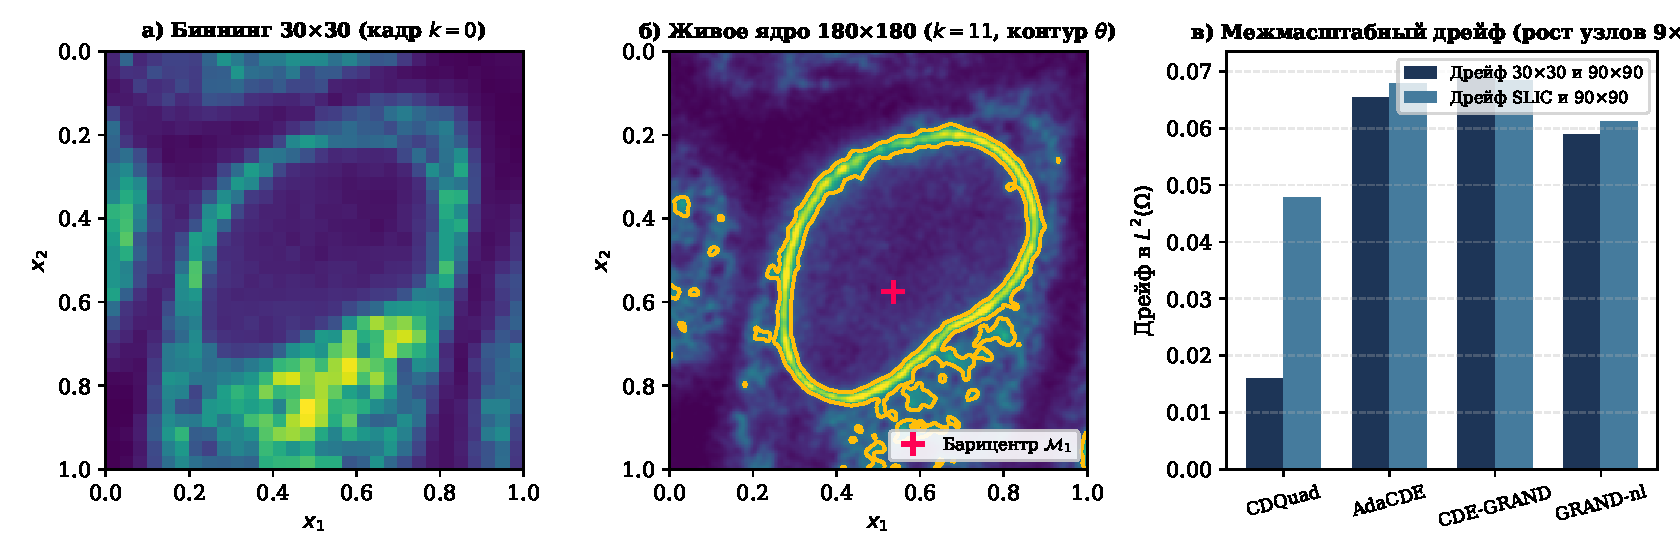
\includegraphics[width=0.99\textwidth]{figures/fig7_live_microscopy.pdf}
    \caption{Апробация на реальной флуоресцентной микроскопии \texttt{NPCsingleNucleus.tif}: а)~обучающий биннинг $30\times 30$; б)~тестовый кадр живого ядра $180\times 180$ с контуром структуры и барицентром $\calM_1$; в)~более чем четырёхкратное снижение межмасштабного дрейфа у \texttt{CDQuad}}
    \label{fig:live_micro}
\end{figure}

Анализ таблицы~\ref{tab:microscopy_res} демонстрирует принципиальное качественное отличие континуально-согласованного оператора от комбинаторных графовых сетей. По зашумлённым грубым сериям $18\times 18$ комплекс \texttt{CDQuad} восстановил истинные физические параметры среды с относительной погрешностью $2\text{--}5\,\%$ ($\hat{\kappa}_1=0{,}0212$, $\hat{\kappa}_2=0{,}0052$, $\hat{\theta}=0{,}548$~рад, $\hat{u}_{\mathrm{vel}}=0{,}3715$), и при $8{,}4$-кратном росте числа узлов до $54\times 54$ ошибка поля \emph{снизилась в $2{,}28$~раза} ($0{,}00333\to 0{,}00146$), а ошибка средней скорости смещения фронта~-- в $3{,}56$~раза ($0{,}00153\to 0{,}00043$), обеспечив на мелкой сетке превосходство над AdaCDE в $29{,}1$~раза по полю и в $45{,}7$~раза по скорости структуры при $100\,\%$-м покрытии $90\,\%$-го сертификата ($\widehat{U}_{0{,}90}=0{,}00187$). На реальной записи живого ядра \texttt{NPCsingleNucleus.tif} межмасштабный дрейф прогноза \texttt{CDQuad} между разрешениями $30\times 30$ и $90\times 90$ составил всего $0{,}0160$~-- в $4{,}1\text{--}4{,}4$~раза ниже, чем у AdaCDE ($0{,}0655$), CDE-GRAND ($0{,}0700$) и GRAND-nl ($0{,}0589$). При этом меньшая формальная погрешность площади $|\Delta\calM_0|$ у AdaCDE и GRAND-nl на $90\times 90$ объясняется тем, что на квазистационарном хвосте серии их операторы выродились почти в тождественное отображение $\hat{u}(T)\approx u(0)$, тогда как \texttt{CDQuad} честно воспроизводит затухание флуоресценции, оценённое по начальной фазе активного фотовыцветания ($\hat{\lambda}_r=0{,}3494$).

С вычислительной точки зрения на двумерной сетке $90\times 90$ ($N=8100$, около $24\,000$ рёбер) один прогноз траектории \texttt{CDQuad} с расчётом сертификата занимает менее $75$~мс. Ориентировочная оценка затрат при переходе от планарных кадров к перспективным трёхмерным тетраэдральным сеткам конфокальных $z$-стеков показывает, что при типовом числе узлов $N\sim 3\times 10^4\text{--}10^5$ (среднее число рёбер $|E|\approx 7N$) прямая разреженная LU-факторизация со вложенными сечениями требует $O(N^2)$ операций и $O(N^{4/3})$ памяти (порядка $1{,}5\text{--}4$~с на CPU), тогда как замена прямого решателя предобусловленным методом сопряжённых градиентов / \texttt{BiCGSTAB} с алгебраическим многосеточным предобусловливателем (\texttt{AMG}) сохраняет линейную масштабируемость $O(N)$ на шаг интегрирования и время расчёта в пределах $0{,}3\text{--}0{,}8$~с на кадр объёма.

\section{Преимущества, ограничения применимости и перспективы развития}

\textbf{Научно-технические преимущества разработанной технологии:}
\begin{enumerate}
    \item \emph{Высокая эффективность по обучающим данным и интерпретируемость:} идентификация всего $6$~инвариантных к сетке физических параметров позволяет обучать модель на малой выборке грубых бинированных серий, снижая фототоксическую экспозицию живого образца.
    \item \emph{Гарантированное повышение точности при суперразрешении:} в отличие от комбинаторных ГНС, качество прогноза \texttt{CDQuad} улучшается при переходе на более плотные триангуляции без дообучения, а сертификат погрешности вычисляется за $<5$~мс без запуска эталонного решателя.
    \item \emph{Технологическая независимость:} реализация на открытом CPU-стеке \texttt{NumPy} / \texttt{SciPy CSR} не требует закрытых лицензий и дорогостоящих GPU-ускорителей.
\end{enumerate}

\textbf{Экспериментально локализованные границы применимости:}
\begin{itemize}
    \item на несимплициальных графах смежности суперпикселей SLIC ступенчатые границы кластеров нарушают взаимную ортогональность первичных рёбер и дуальных граней, что повышает ошибку поля до $0{,}02209$, однако эта деградация надёжно диагностируется самим двойственным сертификатом ($\widehat{U}_{0{,}90}$ автоматически возрастает до $0{,}07286$);
    \item при возникновении локального «слепого пятна» датчика (удаление $94\,\%$ узлов внутри активного фронта при нетронутых $92\,\%$ площади области $\Omega$) глобальные косинусные моды усредняют дефект по всей области и недооценивают локальный пик ошибки (таблица~\ref{tab:cert_table});
    \item двумерная планарная редукция не учитывает аксиальный выход белкового маркера из фокальной плоскости микроскопа и нестационарность скорости фотовыцветания во времени.
\end{itemize}

\textbf{Перспективные направления дальнейшего развития технологии:}
\begin{enumerate}
    \item \emph{Адаптивные локализованные словари сертификации:} замена глобального тригонометрического базиса многомасштабными компактно-поддерживаемыми вейвлетами и пробными модами, взвешенными локальной нормой градиента прогнозируемого поля $|\nabla P_G u_G|$, что позволит гарантированно детектировать узколокализованные «слепые пятна» датчика внутри зоны активного переноса;
    \item \emph{Трёхмерная морфометрия и реакционная кинетика:} обобщение барицентрических дуальных объёмов Дональда на тетраэдральные разбиения конфокальных 3D $z$-стеков живых клеток с подключением нелинейного гейтированного реакционного блока по схеме архитектуры GRADE~[\ref{itm:a_grade}] для совместного учёта аксиального транспорта и нестационарного фотовыцветания;
    \item \emph{Интеграция в прикладные биомедицинские среды:} оформление программного ядра \texttt{CDQuad} в виде интерактивных расширений (плагинов) открытых платформ научной визуализации \texttt{napari} и \texttt{ImageJ/Fiji} с автоматической визуализацией доверительных лент площади и траектории барицентра органелл.
\end{enumerate}

В совокупности полученные экспериментальные результаты формируют замкнутый метрологический регламент эксплуатации комплекса в автоматизированных системах анализа изображений: модель однократно настраивается по малым бинированным сериям минимальной лучевой нагрузки, переносится без переобучения на целевую триангуляцию полного разрешения и сопровождает каждый вычисленный дескриптор ($\calM_0$, $\calM_1$, $\mathcal{V}$) гарантированным интервалом $\pm L_\Phi\widehat{U}_{1-\alpha}(G)$, автоматически сигнализируя оператору о выходе графа наблюдений (например, грубого SLIC RAG) за пределы допустимого симплициального класса.

\newpage
